\chapter{Representation and GAN}

\section{Reviewing}
\begin{enumerate}
\item
When do neural-nets have bad local-minima?
\begin{itemize}
\item
Classical results in \citep{NIPS19951028} show that for unrealizable case, non-linear activation can easily create bad local minima;
\item
Recent results in \citep{ruoyusun2018} show that even for over-parameterized case (thus also realizable), the bad local minima do exist for a class of non-linear activations.
\end{itemize}
\item
People claims that ``over-parametrization'' smooths  the landscape, any rigorous result in this claim?

There are a few rigorous results for this claim. 
For instance, \citep{ruoyusun2018} shows that the loss function of over-parametrized networks has no bad basin (or more precisely, it is a "weakly global" function);
for many smooth enough activations, over-paramterized networks satisfy a stronger geometrical property $PT$ (i.e. at any point, after a tiny generic perturbation, there is a strictly decreasing path from the perturbed point to a global minimum).
\item
How to empirically check nice or bad landscape for any problem (continuous optimization)?

Check values along paths connecting interesting points
\item
When does the neural-nets have enough representation power?

The most important factor is the activation function. It should be bounded and non-constant;
although ReLU is not bounded, it also makes the neural-nets have enough representation power;
but linear/quadratic activation does not.
\end{enumerate}

\section{Representation: depth separation}

\subsection{A simple proof of threhold activation has enough representation power}
Consider the dimension $d=1$ first.
The non-linear activation is $\phi(t)=1\{t\ge0\}$.
It suffices to show that
\[
\overline{\Span\{\phi(at+b)\}} =  \mathcal{C}(\mathcal{D})
\]
for any compact domain $\mathcal{D}\in\mathbb{R}$.
Define the pulse function $\psi(t) = 1\{0\le t<1\}$, which can be expressed as $\psi=\phi(t) - \phi(1-t)$.
It suffices to use the pulse function to approximate any continuous function. 
The general idea is shown in the Figure.~\ref{fig:7:1}.
\begin{figure}[H]
\centering
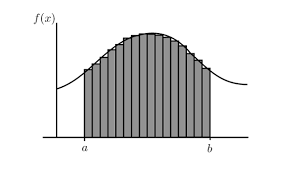
\includegraphics[width=0.7\textwidth]{Seventh_lecture/f_1}
\caption{The pulse function can approximate any continuous function.}
\label{fig:7:1}
\end{figure}
We can see that the insights are very similar to those in Riemann integration, and the proof follows the similar idea as well~\citep[Theorem~(6.4)]{jiewang20191}.

\begin{proof}
Suppose that $\mathcal{D}=[0,1]$ and our target function $f^*\in\mathcal{C}[0,1]$.
The continuity of $f^*$ together with the compactness of $\mathcal{D}$ implies that the function $f^*$ is uniformly continuous, i.e., $\forall\varepsilon>0$, there exists $\delta$ such that for any $|x-x^*|<\delta$, 
\[
|f - f^*|<\varepsilon.
\]
Pick a partition 
\[
\mathcal{P}=\{b_0:=0,b_1=h,b_2=2h,\dots,b_K:=Kh:=1\},\quad
\text{with}~\frac{1}{K}<\Delta.
\]
Therefore, define the approximation function
\[
f(x) = \sum_{i=1}^Ka_i\psi\left(\frac{x-b_i}{b_{i+1} - b_i}\right)\in\Span\{\phi(at+b)\},
\]
where $a_i\triangleq f^*(b_i), i=0,\dots,K-1$.
Then it's easy to verify that $|f(x) - f^*(x)|<\varepsilon$ for any $x\in[0,1]$.
\end{proof}
\begin{remark}
The first step in the proof explains why we need to define the \emph{compact} domain.
\end{remark}

\paragraph{Bibliography}
Then we discuss the representation power for other kinds of activations.
For sigmoid function $\phi(t) = \frac{1}{1+e^{-t}}$, it suffices to show that it can approximate the threshold function very well;
for other types of functions such as switch function, 
some techniques from function analysis are needed.
The paper \citep{3561150} shows that the 
sigmoidal-type activation has enough representation power by using arguments from real analysis;
the paper \citep{Barron1994} further gives an 
mean integrated squared error between the estimated network and a target function $f$, in terms of number of neurons and the input dimension;
the Kolmogorov–Arnold representation theorem actually has solved this problem by using that every multivariate continuous function can be represented as a superposition of continuous functions of one variable, which is also related to Hilbert's thirteenth problem.
The proof in this representation theorem contains the multi-resolution idea, and VCG/Receptor has the similar idea.

\subsection{Depth Separation (Analysis for ReLU Activation)}
It's a common belief that \emph{deep} neural network usually gains better performance. 
We want to analysis this claim from the perspective of representation power.
To show the power of depth, one way is to construct a function represented ``\emph{deep}''-net, then show this function is difficult to be represented by shallow networks.

\begin{enumerate}
\item
Consider a function $\psi$ frequently studied in the dynamical systems literature,
which can be represented with the ReLU activation $\phi$:
\[
\psi(x)=\phi(2\phi(x) - 4\phi(x-0.5)).
\]
\begin{figure}[H]
\centering
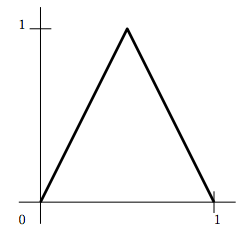
\includegraphics[width=0.4\textwidth]{Seventh_lecture/f_2.png}
\caption{The function $\psi$, which has one ``peak''}
\end{figure}
\item
Construct a function $f^*(x) = \psi^{(L)}(x)$, a the composition of $L$ $\psi$ functions, which has $2^{L-1}$ peaks. See $\psi^{(2)}$ for instance:
\begin{figure}[H]
\centering
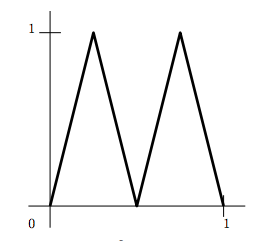
\includegraphics[width=0.4\textwidth]{Seventh_lecture/f_3.png}
\caption{The function $\psi^{(2)}$, which has two ``peaks''}
\end{figure}
\end{enumerate}

It suffices to show $f^*(x) = \psi^{(L)}(x)$ can be represented by deep neural-nets, but it is difficult to be represented by a shallow network, i.e., we need $\mathcal{O}(2^{L})$ neurons of a shallow network for representation.
The intuition is that the 
depth (i.e., function composition) increases oscillation exponentially;
while 
width (i.e., linear combination) increases oscillation linearly.
\begin{definition}
We say that $f$ is $K$-sawtooth if $f$ is piecewise affine with $K$ pieces.
For example, the ReLU function is $2$-sawtooth, and $\psi$ is $4$-sawtooth.
\end{definition}
We can show that function composition is stronger to produce more ``sawtooth'' than addition:
\begin{lemma}
If $f$ is $a$-sawtooth, $g$ is $b$-sawtooth, 
then $f+g$ is at most $(a+b)$-sawtooth, $f\circ g$ is at most $ab$-sawtooth.
\end{lemma}
By using this lemma, we can show the converse error bound on the representation power of shallow network:
\begin{theorem}\label{The:7:2}
Given an underlying function $F$ and data points $\{(x_i,y_i\triangleq F(x_i))\}_{i=1}^n, y_i\in\{0,1\}$, define the classification error for the approximation function $f$:
\[
R(f) = \frac{1}{n}\sum_{i=1}^n1\left\{
\text{sign}(f(x_i) - 1/2)\ne y_i
\right\}.
\]
Construct the data points $x_i=\frac{i}{2^{L^*}}$, $y_i=\psi^{(L^*)}(x_i), i=1,\dots,2^{L^*}$. As a result, $y=(0,1,0,1,\dots)$, and $F(x) = \psi^{(L^*)}(x)$.
If a ReLU neural network $f$ has $L$ layers, and width $m<2^{(L^*-k)/L-1}$, then
$R(f)>\frac{1}{2}-\frac{1}{3}\frac{1}{2^{k-1}}$.
\end{theorem}

\begin{corollary}
If $f$ has $L$ layers with width $m<2^{(L^*-1)/L-1}$, then the error function is lower bounded by a constant: $R(f)>1/6$.
\end{corollary}

\begin{corollary}
If $f$ has no more than $\sqrt{L^*}$ layers, then we need at least $m>2^{\mathcal{O}(\sqrt{L^*})}$ neurons to get the error less than $1/6$.
\end{corollary}


%idea: information-theoretical view of depth separation.
\begin{remark}
There is an Implicit assumption on Theorem~(\ref{The:7:2}), i.e., the neural network is fully connected feedforward.
It does not apply to ResNet and RNN.
The paper \citep{NIPS2018_7855} shows the representation power for ResNet.
\end{remark}
\begin{remark}
The representation power on other kinds of neural-nets is a popular problem, such as graph neural-nets and meta-learning.
\end{remark}

\paragraph{Summarization}
There are three criteria for the performance of neural-nets:
\[
\left\{
\begin{aligned}
\text{Representation Error}\\
\text{Optimization Error}\\
\text{Generalization Error}
\end{aligned}
\right.
\]
The important factors for the success of neural-nets are as follows:
\begin{enumerate}
\item
The depth of neural-nets relates to the representation error;
\item
The width of neural-nets relates to the landscape of neural-nets, which further influences the optimization error;
\item
The initialization and normalization techniques relate to the convergence performance of optimization;
\item
The architecture design influences the representation error;
and the optimization error;
\item
The SGD algorithm influences the speed for convergence during the optimization process, and people believe that it also tends to give a solution with low generalization error
\end{enumerate}
\begin{remark}
Why the over-parametrization of neural-nets usually do not lead to over-fitting?
Prof. Ruoyu Sun gives his understanding of this question.
Consider true data $\{(x_i,y_i)\}_{i=1}^n$ generated by $f^*(x_i) = y_i$.
We want to approximate $f^*$ with $f$, by using these $n$ data points.
Let $W^*$ denote the representation-power threshold, and $n^*$ denotes the threshold for the number of data points, under which the approximation is likely to be bad.
The number of parameters of $f$ is more than $W^*$ will not cause over-fitting, 
but when $n<n^*$, it is likely to cause over-fitting.
\end{remark}

\section{GAN}
Now we turn from supervised learning to unsupervised learning. Prof. Ruoyu Sun will give basic formulation about GAN this lecture, and Prof. Mingyi Hong will provide the introduction to  Adversarial Attack $\&$ Defense in the next lecture.

\paragraph{Motivation}
\begin{quotation}{Richard Feymann:}
What I cannot create, I do not understand
\end{quotation}
We wish to learn the data distribution $\mathbb{P}_d$, e.g., a style of writing of articles.
In order to do so, we build a generative model which generates $\mathbb{P}_g$, e.g., imitates writing articles;
and a classifier which judges whether the received sample comes from $\mathbb{P}_d$ or $\mathbb{P}_g$, e.g., give comments to the written samples.
Finally, we want $\mathbb{P}_g\approx\mathbb{P}_d$, e.g., the generated article has a similar style of the original one.

We are interested in solving the optimization problem 
\[
\min_{\mathbb{P}_g}\Phi(\mathbb{P}_d,\mathbb{P}_g)
\]
The question is that what distance measure should the $\Phi$ be?
Statiscians tend to pick $\Phi(P,Q)=\text{KL}(P,Q)$ or $\Phi(P,Q)=\text{JS}(P,Q)$ empirically.
However, it is not clear whether these distance metrics are good metrics. An ideal metric should satisfy the following property: if two images are from the same class, then their distance is small; if they are from different classes, then their distance is large. Is the JS distance between the images of two cats is smaller than the distance between a cat and a dog? This is not clear. The major issue here is that common distances may not capture the right representation of the images. To explain the solution, next, we use an example of fake paintings.
\paragraph{Discussion}
Suppose we want to generate an appropriate painting, denoted as $X$.
Given an artist paint something, denoted as $\hat{X}$;
and hire a critic to judge whether it is good or bad. 
We use $D(x)$ to represent the probability that the input $x$ is thought by the critic to come from the data $P_d$ rather than $P_g$.
The evaluation score can be modeled as
\[
L^{\text{GAN}}(\mathbb{P}_d,D)=
\mathbb{E}_{x\sim \mathbb{P}_d}[\log D(x)]
+
\mathbb{E}_{\hat{x}\sim \mathbb{P}_g}[\log(1-D(\hat{x}))]
\]
Pick the \emph{best} critic, i.e., the most strict critic, the distance measure is 
\[
\Phi(\mathbb{P}_d,\mathbb{P}_g)
=
\max_{D}
L^{\text{GAN}}(\mathbb{P}_d,D)
\]
Therefore, the optimization for GAN is a minimax problem:
\begin{equation}\label{Eq:7:1}
\min_{\mathbb{P}_g}\max_{D}\mathbb{E}_{x\sim \mathbb{P}_d}[\log D(x)]
+
\mathbb{E}_{\hat{x}\sim \mathbb{P}_g}[\log(1-D(\hat{x}))]
\end{equation}
When proposing a new mode, the sanity-check is needed, i.e., 
ensure that the global optimum equals whatever we want, i.e., 
the optimal solution $\mathbb{P}_g^*=\mathbb{P}_d$.
\begin{theorem}[\citep{NIPS2014_5423}]
The global minimum of the problem (\ref{Eq:7:1}) is achieved if and only if $\mathbb{P}_g^*=\mathbb{P}_d$. Moreover, this optimization problem is equivalent to minimizing the Jensen-Shannon divergence
\[
\Phi(\mathbb{P}_g,\mathbb{P}_d)
=-\log 4+2\text{JSD}(\mathbb{P}_d\|\mathbb{P}_g).
\]
\end{theorem}
\begin{proof}
Finding the global minima of the problem consists of two steps: 
first, we need to specify the range of the objective function; 
second, we need to identify some points that achieve the extreme of the range. 
\begin{itemize}
\item
Question 1: What is the range of the objectvie function?

We find that $D(x)\in(0,1)$, and therefore $L^{GAN}\in(-\infty,0)$.
It seems that it is meanless to solve an optimization problem with negative infinite value.
In fact, the objective is lower bounded since the maximum criteria help.
\item
Question 2: Check when does the objective achieve the optimum.

Consider the finite support distribution for simplicity.
Denote the pmf from $\mathbb{P}_d$ and $\mathbb{P}_g$ as $\{q_1,\dots,q_n\}$, $\{p_1,\dots,p_n\}$, respectively.
It suffices to solve
\[
\begin{array}{ll}
\min_{p\in \mathcal{P}^n}\max_{d_i\in(0,1)}&\sum_{i=1}^nq_i\log d_i + \sum_{i=1}^np_i\log(1-d_i)\\
\text{with}&\mathcal{P}^n=\{p\mid \sum_ip_i=1,p_i\ge0\}
\end{array}
\]
Consider the maximum optimization first:
\[
\max_{d_i\in(0,1)}\sum_{i=1}^nq_i\log d_i + \sum_{i=1}^np_i\log(1-d_i)
\]
It is decomposable in terms of $i$. For each single problem $\max_{d_i}q_i\log d_i + p_i\log(1-d_i)$, we find the optimal solution is $d_i = \frac{q_i}{q_i+p_i}$.
Substituting this solution into $\Phi(\mathbb{P}_g,\mathbb{P}_d)$, we imply
\begin{align*}
\Phi(q,p) &= \sum_iq_i\log\frac{q_i}{q_i+p_i}+
 \sum_ip_i\log\frac{p_i}{q_i+p_i}\\
 &=\text{JSD}(p\| q)-2\log 2
\end{align*}
We find that it suffices to minimize $\Phi(q,p) \in(-2\log 2,0)$, which is a valid probem now.
After solving this minimization problem, we obtain the optimal $d$:
\[
d_i^*(p_i) = \frac{q_i}{q_i+p_i}=\left\{
\begin{aligned}
1,&\quad\text{if $p_i=0$, juage as a bad generator}\\
0,&\quad\text{if $q_i=0,p_i>0$, juage as invalid}\\
1/2,&\quad\text{juage as a good generator}
\end{aligned}
\right.,
\] 
i.e.,
for certain data point $i$, the discrimintator returns a probability $q_i/(q_i+p_i)$.
At optimal $p^*=q$, $d_i^*(p^*)=1/2,\forall i$.
\end{itemize}
%
%\begin{itemize}
%\item
%Question 1: What are the gobal minima?
%\begin{itemize}
%\item
%Question 1.1: What is the range of the objectvie function?
%We find that $D(x)\in(0,1)$, and therefore $L^{GAN}\in(-\infty,0)$.
%It seems that it is meanless to solve an optimization problem with negative infinite value.
%In fact, the objective is lower bounded since the maximum criteria help.
%\item
%Question 1.2: Check when does the objective achieve the optimum.
%Denote the pmf from $\mathbb{P}_d$ and $\mathbb{P}_g$ as $\{q_1,\dots,q_n\}$, $\{p_1,\dots,p_n\}$, respectively.
%It suffices to solve
%\[
%\begin{array}{ll}
%\min_{p\in \mathcal{P}^n}\max_{d_i\in(0,1)}&\sum_{i=1}^nq_i\log d_i + \sum_{i=1}^np_i\log(1-d_i)\\
%\text{with}&\mathcal{P}^n=\{p\mid \sum_ip_i=1,p_i\ge0\}
%\end{array}
%\]
%Consider the maximum optimization first:
%\[
%\max_{d_i\in(0,1)}\sum_{i=1}^nq_i\log d_i + \sum_{i=1}^np_i\log(1-d_i)
%\]
%It is decomposable in terms of $i$. For each single problem $\max_{d_i}q_i\log d_i + p_i\log(1-d_i)$, we find the optimal solution is $d_i = \frac{q_i}{q_i+p_i}$.
%Substituting this solution into $\Phi(\mathbb{P}_g,\mathbb{P}_d)$, we imply
%\begin{align*}
%\Phi(q,p) &= \sum_iq_i\log\frac{q_i}{q_i+p_i}+
% \sum_ip_i\log\frac{p_i}{q_i+p_i}\\
% &=\text{JSD}(p\| q)-2\log 2
%\end{align*}
%We find that it suffices to minimize $\Phi(q,p) \in(-2\log 2,0)$, which is a valid probem now.
%After solving this minimization problem, we obtain the optimal $d$:
%\[
%d_i^*(p_i) = \frac{q_i}{q_i+p_i}=\left\{
%\begin{aligned}
%1,&\quad\text{if $p_i=0$, juage as a bad generator}\\
%0,&\quad\text{if $q_i=0,p_i>0$, juage as invalid}\\
%1/2,&\quad\text{juage as a good generator}
%\end{aligned}
%\right.,
%\] 
%i.e.,
%for certain data point $i$, the discrimintator returns a probability $q_i/(q_i+p_i)$.
%At optimal $p^*=q$, $d_i^*(p^*)=1/2,\forall i$.
%\end{itemize}
%\end{itemize}
\end{proof}

\begin{remark}
This result is misleading somehow. 
For instance, images are continuous distributions,
so it is impossible to expect the generated image exactly match the original image, i.e., 
we can never achieve values for $d_i$ other than $\{0,1\}$.
\end{remark}
\begin{remark}
This proof justifies GAN by relating it to Jensen–Shannon divergence, but in the beginning we think that this distance is not good. 
\end{remark}

\paragraph{Motivation of W-GAN}
The Jensen–Shannon divergence is not a good metric in some settings.
For instance, it is impossible to measure the distance between two distributions with the different supporting set, but Wasserstein distance givens a reasonable measure. 
The $p$-th Wasserstein distance between two probability measures $\mu,\nu$ is defined as
\[
W_p(\mu,\nu)=\min_{p\sim\Gamma(\mu,\nu)}\left(\mathbb{E}_{(x,y)\sim\mathcal{P}}|x-y|^p\right)^{1/p}
\]
where $\Gamma(\mu,\nu)$ denotes the set of all couplings of $\mu$ and $\nu$.
When $p=1$, finding the Wasserstein distance reduces to solving an LP problem.
Moreover, the $W_1$ distance can be re-expressed using duality of LP:
\[
W_1(\mu,\nu)=\sup_{|f|_L\le1}
\mathbb{E}_{x\sim\mu}[f(x)]
-
\mathbb{E}_{y\sim\nu}[f(y)]
\]
where the supremum is taken over all the $1$-Lipschitz functions $f$.
The W-GAN solves the following problem:
\[
\min_{\mathbb{P}_g}\max_{|f|_L\le1}
\mathbb{E}_{x\sim\mu}[f(x)]
-
\mathbb{E}_{\hat{x}\sim\nu}[f(\hat{x})]
\]
\begin{remark}
The origin GAN using Jensen–Shannon divergence also works, but using Wasserstein distance is better. However, Wasserstein distance does has some disadvantages.
For example, it is not generalizable, i.e., to approximate $W_1(\mu,\nu)$, we require $\exp(d)$ samples from $(\mu,\nu)$, where $d$ is the supporting dimension of $\mu$ and $\nu$, even when they are Gassuain distributions.
One solution is to realize that the objective functions in the original GAN and W-GAN are actually using different distance metrics called "neural network distance". Again, we emphasize that neural-network distance is not a new distance, but a distance with good generalization property, and is used by everyone although the distance metric is not explicitly defined before.

\end{remark}
























